\documentclass[11pt]{ctexart}

\usepackage[a4paper,margin=1in]{geometry}
\usepackage{amsmath,amssymb,amsfonts}
\usepackage{booktabs}
\usepackage{graphicx}
\usepackage{array}
\usepackage{siunitx}
\usepackage{hyperref}
\usepackage{enumitem}
\usepackage{caption}
\usepackage{longtable}

\hypersetup{colorlinks=true,linkcolor=black,citecolor=black,urlcolor=black}
\sisetup{round-mode=places,round-precision=4,detect-weight=true,detect-family=true}

\title{????????????????????????????????}
\author{????????????}
\date{}

\begin{document}
\maketitle

\begin{abstract}
????????????????????????????????????????????????????????????????????????????????????????????????????????????????????????????????????????????????????????????????????????????????????????????????????????????????????????????????? horizon ? seed ?????????????????????????????????????? METR-LA ???????????????paper-inspired GraphWaveNetFull ??? 15?30 ? 60 ???????????? MAE??? LastValue ??????? 0.5539?0.6438 ? 0.8986???????????????????? identity graph?? physical?correlation ? adaptive graph ?????????????? horizon ?????????? SOTA???????????????????????????????????????????????????????????????????????????????
\end{abstract}

\textbf{????} ?????????????Graph WaveNet?STGCN?METR-LA?????????????????

\section{??}
??????????????????????????????????????????????????????????? LastValue ????????????????????????????????????????????????????????????????????????????????????????????????

????????????????????????????????????????????? baseline ???????????????????????? horizon???????????? synthetic demo ???????????????? Agent ?????????????????????????????????????????????????????????????????????

??????? \emph{Urban Traffic Forecasting \& Congestion Analysis Agent}??????????????????????????????????????????????????????????????????????????????????????????????????????????????????????????
\begin{itemize}[leftmargin=*]
  \item ?? METR-LA ??????????????? HDF5 ???????DCRNN ??????????????????????????
  \item ??????????????????????temporal-only ?????educational lite ???? paper-inspired full ????
  \item ?? GraphWaveNetFull ? STGCNFull????????????????????????????????????????????
  \item ??? horizon?? seed ??????????????? MAE?RMSE?raw MAPE ? masked MAPE?????????? MAE?RMSE ? masked MAPE?
  \item ?????????????????????? identity?physical?correlation ? adaptive graph ???????? low speed?speed drop?high variance ? normal flow ?????????
  \item ????????????????????????????????????????????????????
\end{itemize}

\section{????}
??????????????? $G=(V,E,A)$????$V$ ?? $N$ ?????????$E$ ????????????????$A\in\mathbb{R}^{N\times N}$ ?????????? $t$??????? $X_t\in\mathbb{R}^{N\times F}$??? $F$ ???????? METR-LA ??????????????

????? $T$ ????????
\begin{equation}
  X_{t-T+1:t}=\{X_{t-T+1},\ldots,X_t\}\in\mathbb{R}^{T\times N\times F},
\end{equation}
???????? $H$ ????????
\begin{equation}
  \hat{Y}_{t+1:t+H}=f_\theta(X_{t-T+1:t}, A)\in\mathbb{R}^{H\times N}.
\end{equation}
????? $T=12$??? 5 ????????? 60 ?????$H\in\{3,6,12\}$??????? 15?30 ? 60 ?????

??????????????????????????????????????????????????????????????????????????????????? 70\%/10\%/20\% ?????????????????? forward fill?backward fill ???????????????????????????????

\section{????}
???????????????????????????????

\subsection{???}
??????? synthetic demo ????? METR-LA/PEMS-BAY ?????Synthetic ??????????????? CI smoke test???????????????????????????????? HDF5 ????? DCRNN ?? \texttt{adj\_mx.pkl} ?????

????????????? $i$ ??????????? $i$ ??? $i$ ??????? HDF5 DataFrame ????? \texttt{adj\_mx.pkl} ? sensor ids ???????????????????????????????????????????????????????????????? \texttt{node\_alignment\_report.json}??????????????????

\subsection{?????}
??????????????????????????????????????????temporal-only ?????????????????????lite ?????????????full ?????????????????????????

\subsection{???}
???????????????????????????????????????? 0 ? raw MAPE ?????????? MAE?RMSE ? masked MAPE ?????????

\subsection{????}
???????????????????Agent ??????????????? metrics?summary?ablation?congestion subset ????????????????? trace?Agent ??????????????????????

\subsection{????}
?????? Dashboard ????????????horizon ??????????????????????????????? CSV ????????????

\section{????}
\subsection{?????????}
\textbf{LastValue} ?????????????????????????????????????????LastValue ?????????????????

\textbf{HistoricalAverage} ???????????????\textbf{SeasonalNaive} ?????? time-of-day ?????????????????? HistoricalAverage??????????HistoricalAverage ? SeasonalNaive ?????????????????????????????

\subsection{Temporal-only ????}
LSTM ? GRU ???????? flatten ???????????????????????????????????????????????

\subsection{Educational Lite ???}
STGCNImproved ? GraphWaveNetLite ????????????? temporal module ? graph module ??????????????????????????

\subsection{Paper-inspired GraphWaveNetFull}
GraphWaveNetFull ?? Graph WaveNet ?????????? start convolution?dilated causal temporal convolution?gated activation?diffusion graph convolution?residual connection?skip connection?end convolution ? adaptive adjacency????????????
\begin{equation}
  Z' = \tanh(\Theta_f * Z) \odot \sigma(\Theta_g * Z),
\end{equation}
?? $*$ ???????$\odot$ ????????Adaptive adjacency ???????????
\begin{equation}
  A_{adaptive}=\operatorname{softmax}(\operatorname{ReLU}(E_1E_2)).
\end{equation}
???????????? paper-inspired ????????? Graph WaveNet ???

\subsection{Paper-inspired STGCNFull}
STGCNFull ?? ST-Conv block ???? TemporalConv?GraphConv?TemporalConv ????????? residual connection?layer normalization ? dropout???????? Chebyshev-style $K$ ???????????????????????????????

\section{????}
\subsection{???}
???? METR-LA ??????????? 207 ?????????????????? $[T,N,F]$??? $N=207$?$F=1$???????? DCRNN ??????????????????? HDF5 ????????

\subsection{????}
RTX 5090 ???? batch size 64????? 100 epoch???? 0.001?weight decay $10^{-4}$?early stopping patience ? 20?gradient clipping norm ? 5.0??? CUDA ????? AMP mixed precision?????? $H\in\{3,6,12\}$ ? seed $\{42,43,44\}$ ???????

\subsection{????}
???? MAE?RMSE ? masked MAPE?
\begin{align}
  \operatorname{MAE} &= \frac{1}{M}\sum_i |y_i-\hat{y}_i|,\\
  \operatorname{RMSE} &= \sqrt{\frac{1}{M}\sum_i (y_i-\hat{y}_i)^2},\\
  \operatorname{masked\ MAPE} &= \frac{100}{|\Omega|}\sum_{i\in\Omega}\left|\frac{y_i-\hat{y}_i}{y_i}\right|.
\end{align}
?? $\Omega$ ???????? 0 ????Raw MAPE ???????????????

\section{?????}
?~\ref{tab:main_results_cn} ??? METR-LA ?? seed ?????GraphWaveNetFull ? 15?30 ? 60 ???? horizon ?????? MAE???? STGCNFull ? GraphWaveNetLite?LastValue ????????????????????????????????

\begin{table}[htbp]
\centering
\caption{METR-LA ? seed ??????????????}
\label{tab:main_results_cn}
\begin{tabular}{llrrrr}
\toprule
???? & ?? & MAE & RMSE & masked MAPE & ??? \\
\midrule
15 ?? & GraphWaveNetFull & 2.9578 & 8.0756 & 6.5940 & 732335 \\
15 ?? & STGCNFull & 3.0951 & 8.3104 & 7.1515 & 186115 \\
15 ?? & GraphWaveNetLite & 3.1175 & 8.0813 & 7.2675 & 56611 \\
15 ?? & STGCNImproved & 3.2775 & 8.2346 & 7.4561 & 58307 \\
15 ?? & LastValue & 3.5117 & 8.5862 & 8.1707 & 0 \\
\midrule
30 ?? & GraphWaveNetFull & 3.5862 & 9.7628 & 7.7682 & 733874 \\
30 ?? & STGCNFull & 3.7471 & 9.9593 & 8.6012 & 186310 \\
30 ?? & GraphWaveNetLite & 3.7923 & 9.7942 & 8.7781 & 56806 \\
30 ?? & STGCNImproved & 3.9764 & 10.0656 & 8.8803 & 58502 \\
30 ?? & LastValue & 4.2301 & 10.3986 & 9.7409 & 0 \\
\midrule
60 ?? & GraphWaveNetFull & 4.5384 & 11.8601 & 9.6252 & 736952 \\
60 ?? & STGCNFull & 4.7723 & 12.2233 & 10.7236 & 186700 \\
60 ?? & GraphWaveNetLite & 4.8819 & 12.1295 & 11.2626 & 57196 \\
60 ?? & STGCNImproved & 5.1507 & 12.4042 & 11.5666 & 58892 \\
60 ?? & LastValue & 5.4370 & 12.9603 & 12.3455 & 0 \\
\bottomrule
\end{tabular}
\end{table}

?? LastValue?GraphWaveNetFull ? 15?30?60 ???????? MAE ???? 0.5539?0.6438 ? 0.8986??? LastValue ??????????????????????????????????????????????????????????????? METR-LA ?????????????????????????????

\begin{figure}[htbp]
  \centering
  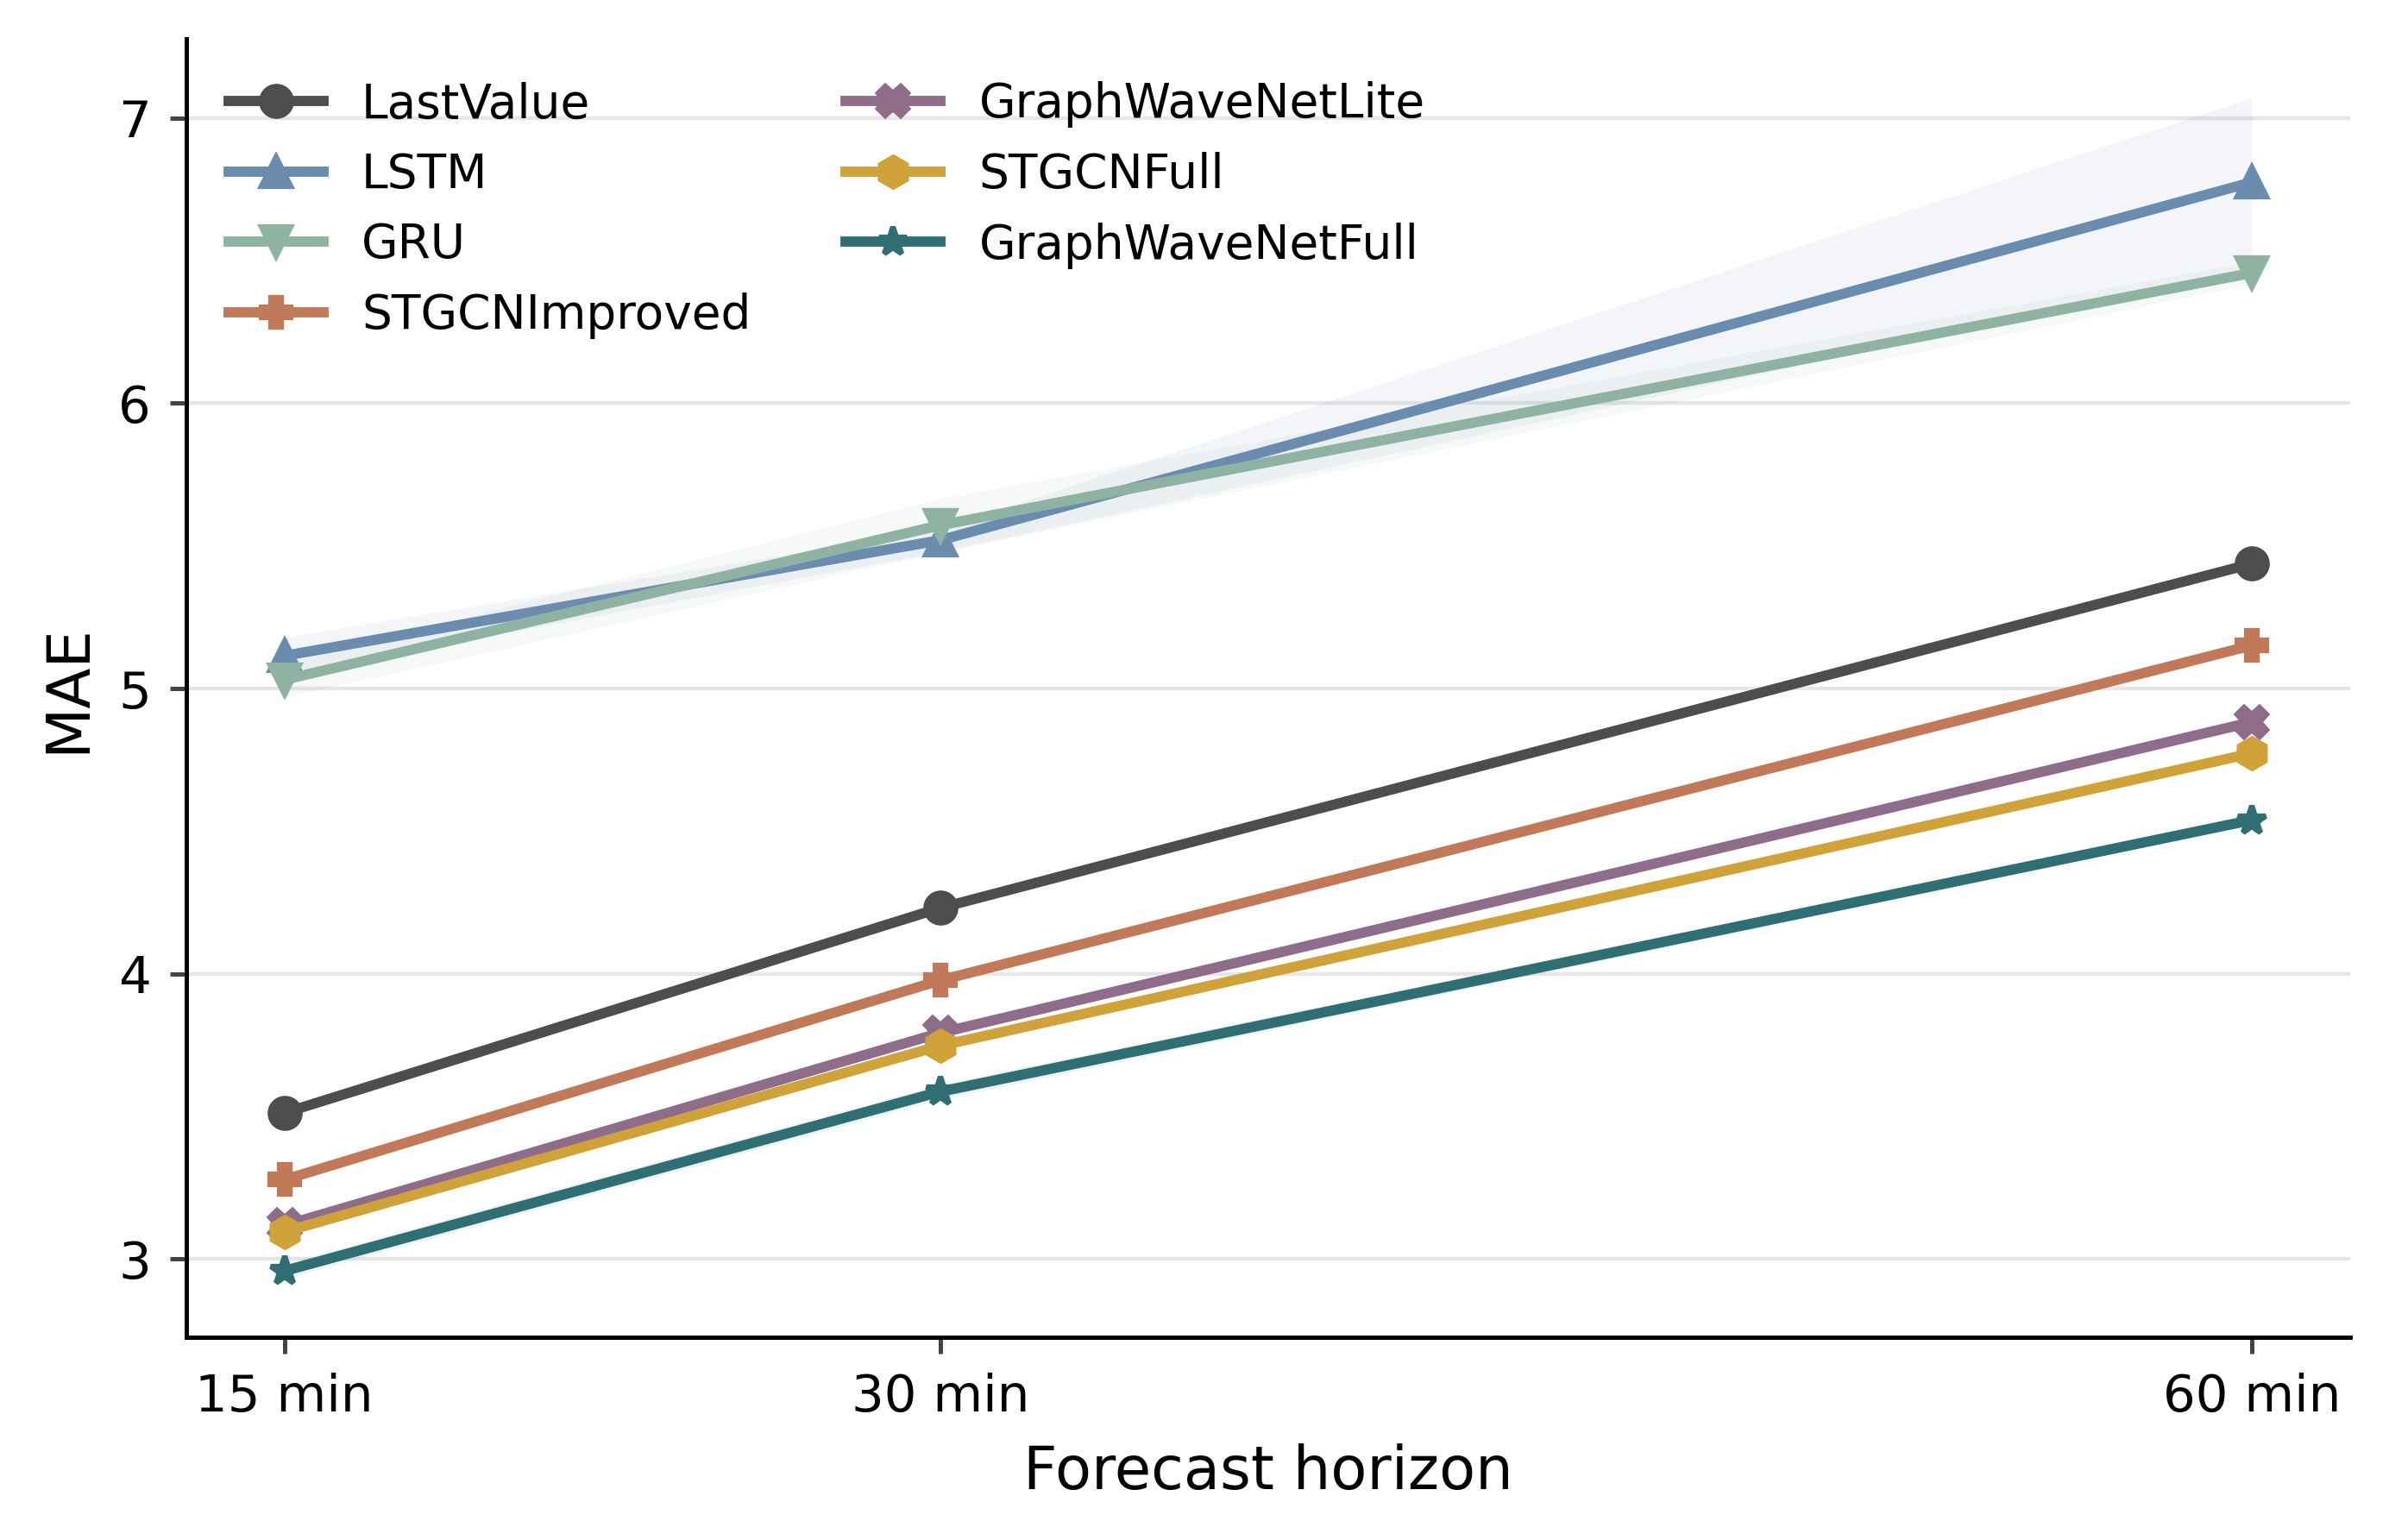
\includegraphics[width=0.82\linewidth]{../experiments/figures/METR-LA_MAE_by_Horizon.png}
  \caption{???? horizon ?? MAE?}
  \label{fig:mae_horizon_cn}
\end{figure}

\begin{figure}[htbp]
  \centering
  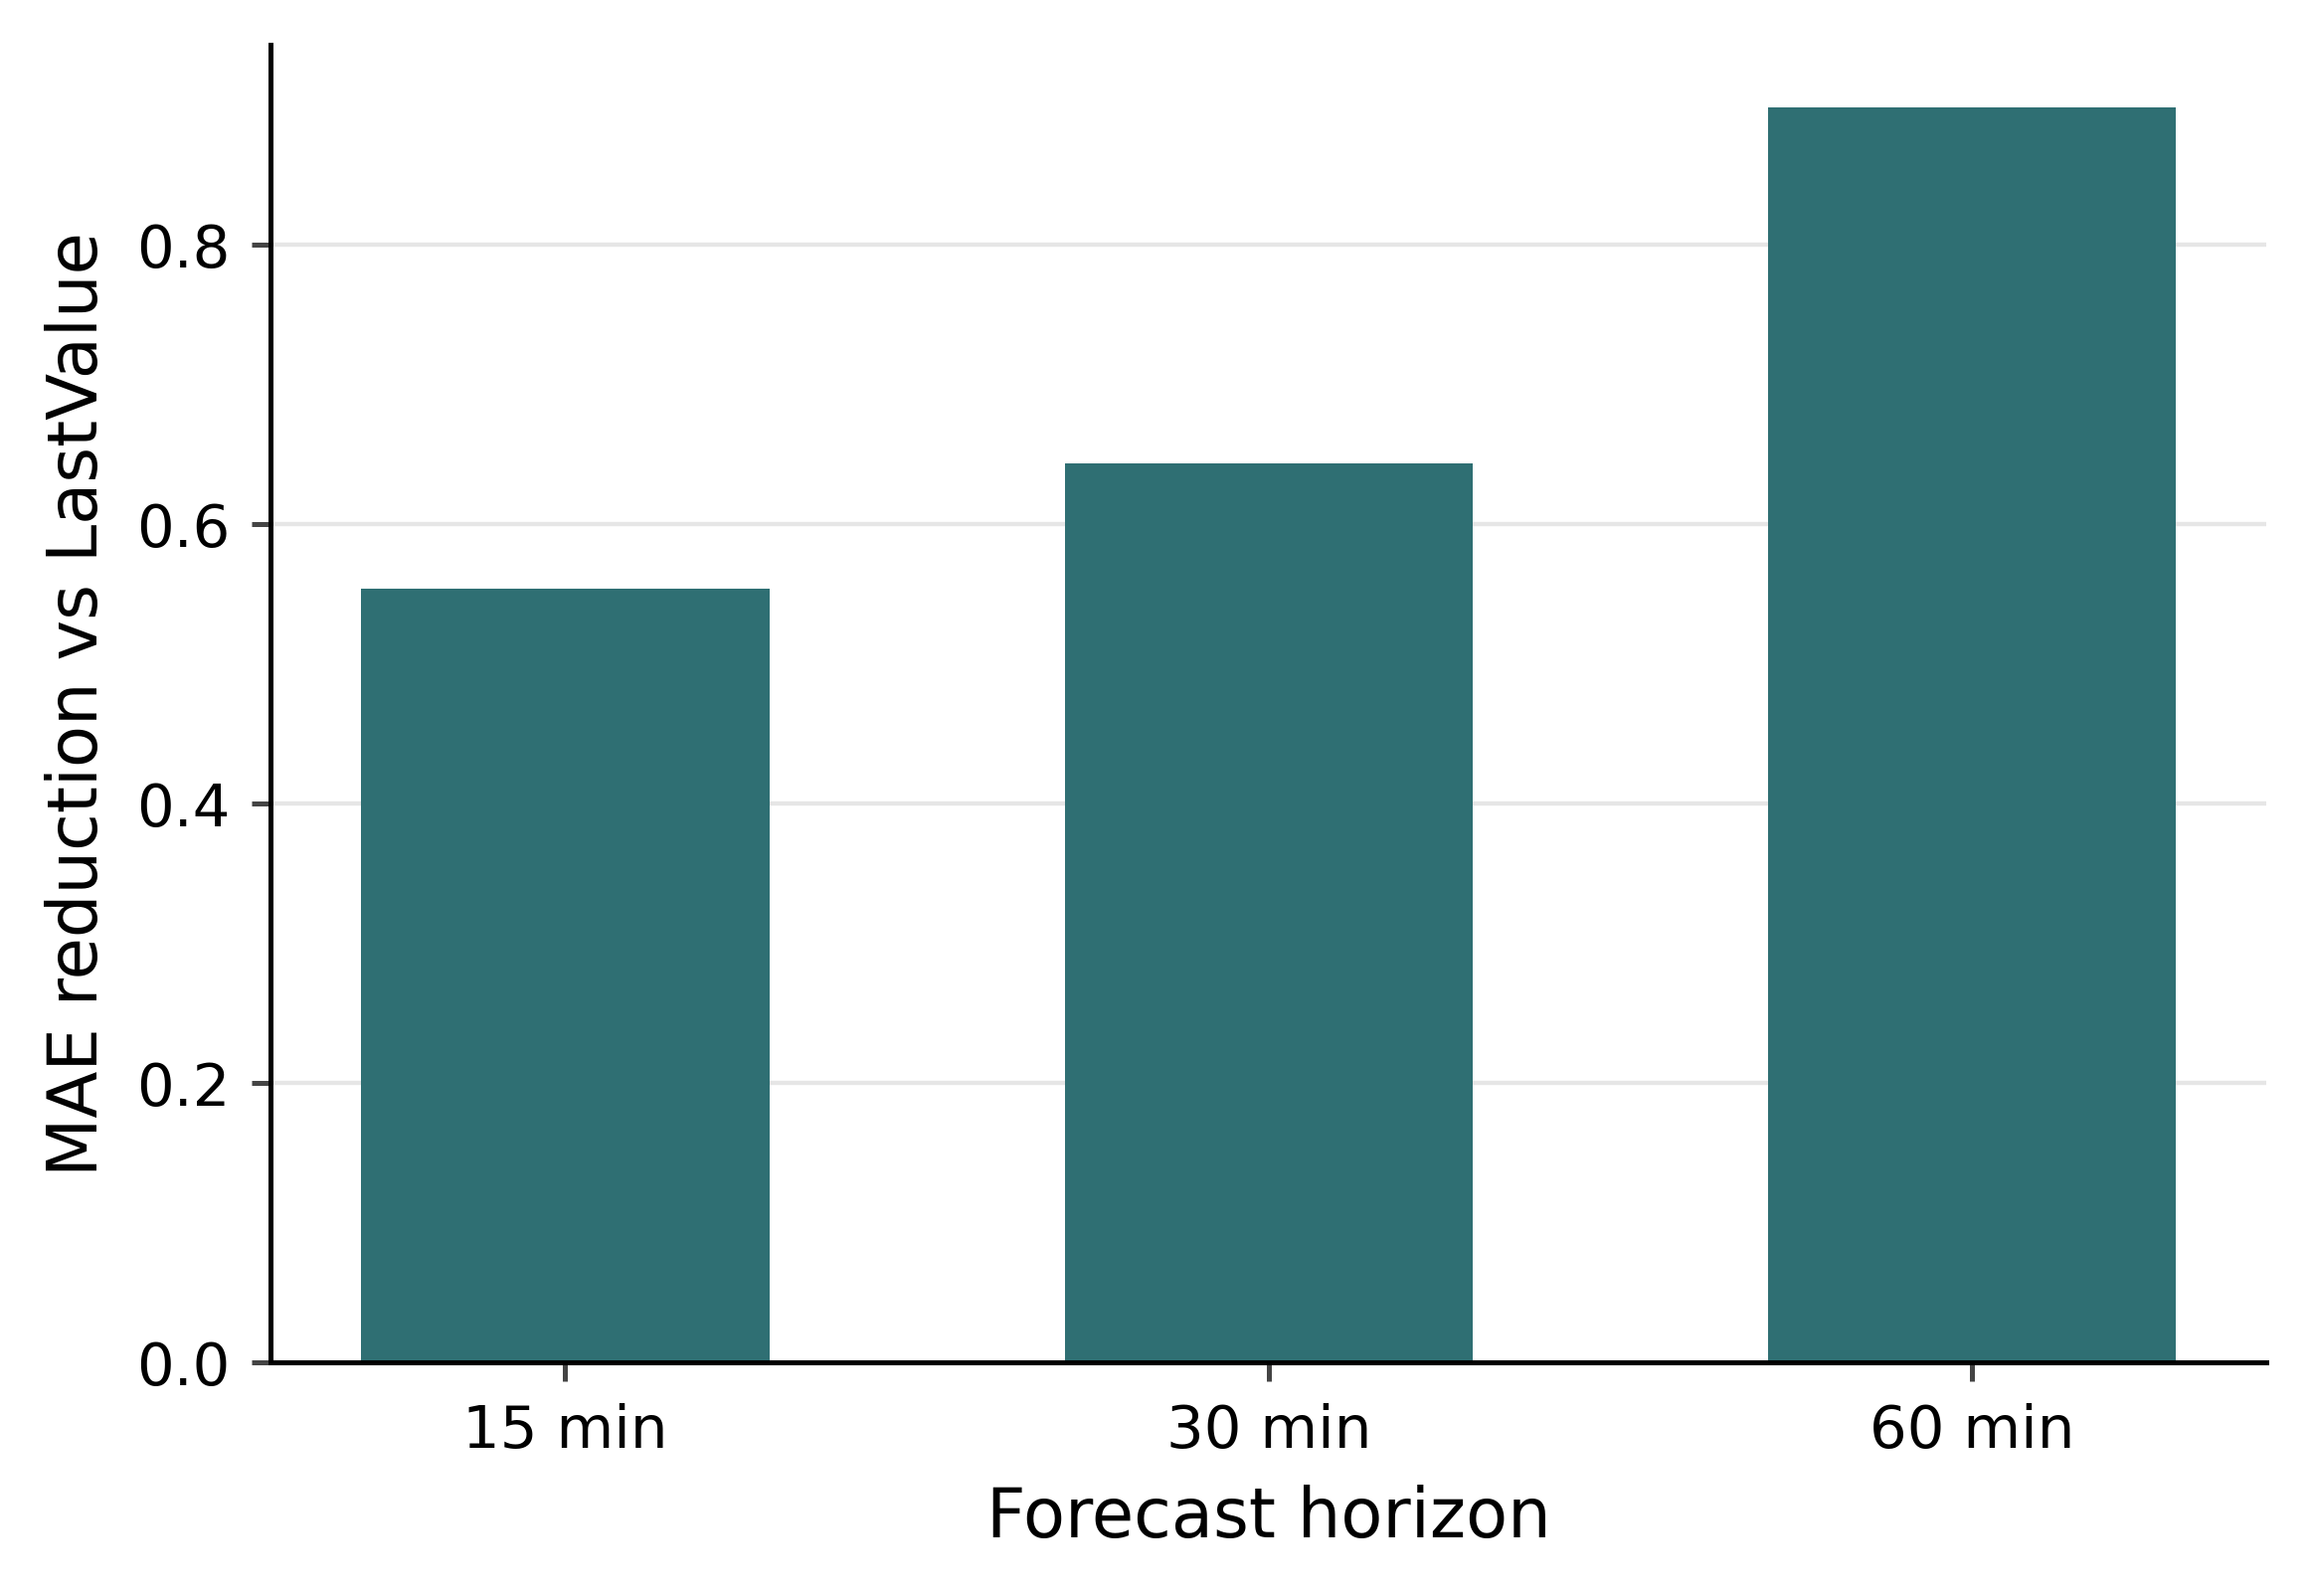
\includegraphics[width=0.82\linewidth]{../experiments/figures/GraphWaveNetFull_MAE_Reduction_vs_LastValue.png}
  \caption{GraphWaveNetFull ?? LastValue ? MAE ???}
  \label{fig:mae_reduction_cn}
\end{figure}

\section{???????}
??????????????????????????????? identity?physical?correlation ? adaptive ??????Identity graph ?????????????physical graph ?????????correlation graph ???????????????????????adaptive graph ???????????????????????

?~\ref{tab:ablation_cn} ???????? horizon ? MAE ???????GraphWaveNetFull ??? horizon ??? adaptive/physical ???????STGCNFull ? 15 ? 30 ????? physical ???? 60 ????? correlation ???STGCNImproved ??????? physical graph?GraphWaveNetLite ????? correlation ???

\begin{table}[htbp]
\centering
\caption{?????????? horizon ???????}
\label{tab:ablation_cn}
\begin{tabular}{llrrr}
\toprule
?? & ????? & ???? & MAE & masked MAPE \\
\midrule
GraphWaveNetFull & adaptive/physical & 15 ?? & 2.9683 & 6.6080 \\
GraphWaveNetFull & adaptive/physical & 30 ?? & 3.5881 & 7.8489 \\
GraphWaveNetFull & adaptive/physical & 60 ?? & 4.5191 & 9.6320 \\
GraphWaveNetLite & correlation & 15 ?? & 3.1068 & 7.2337 \\
GraphWaveNetLite & correlation & 30 ?? & 3.7703 & 8.7044 \\
GraphWaveNetLite & correlation & 60 ?? & 4.8106 & 11.0375 \\
STGCNFull & physical & 15 ?? & 3.0910 & 7.1828 \\
STGCNFull & physical & 30 ?? & 3.7561 & 8.6168 \\
STGCNFull & correlation & 60 ?? & 4.7425 & 10.4494 \\
STGCNImproved & physical & 15 ?? & 3.2766 & 7.4292 \\
STGCNImproved & physical & 30 ?? & 3.9764 & 8.9074 \\
STGCNImproved & physical & 60 ?? & 5.1441 & 11.5140 \\
\bottomrule
\end{tabular}
\end{table}

?????????????????????????????????????????????????????????????????????????????????????????????????????? horizon ???????

\begin{figure}[htbp]
  \centering
  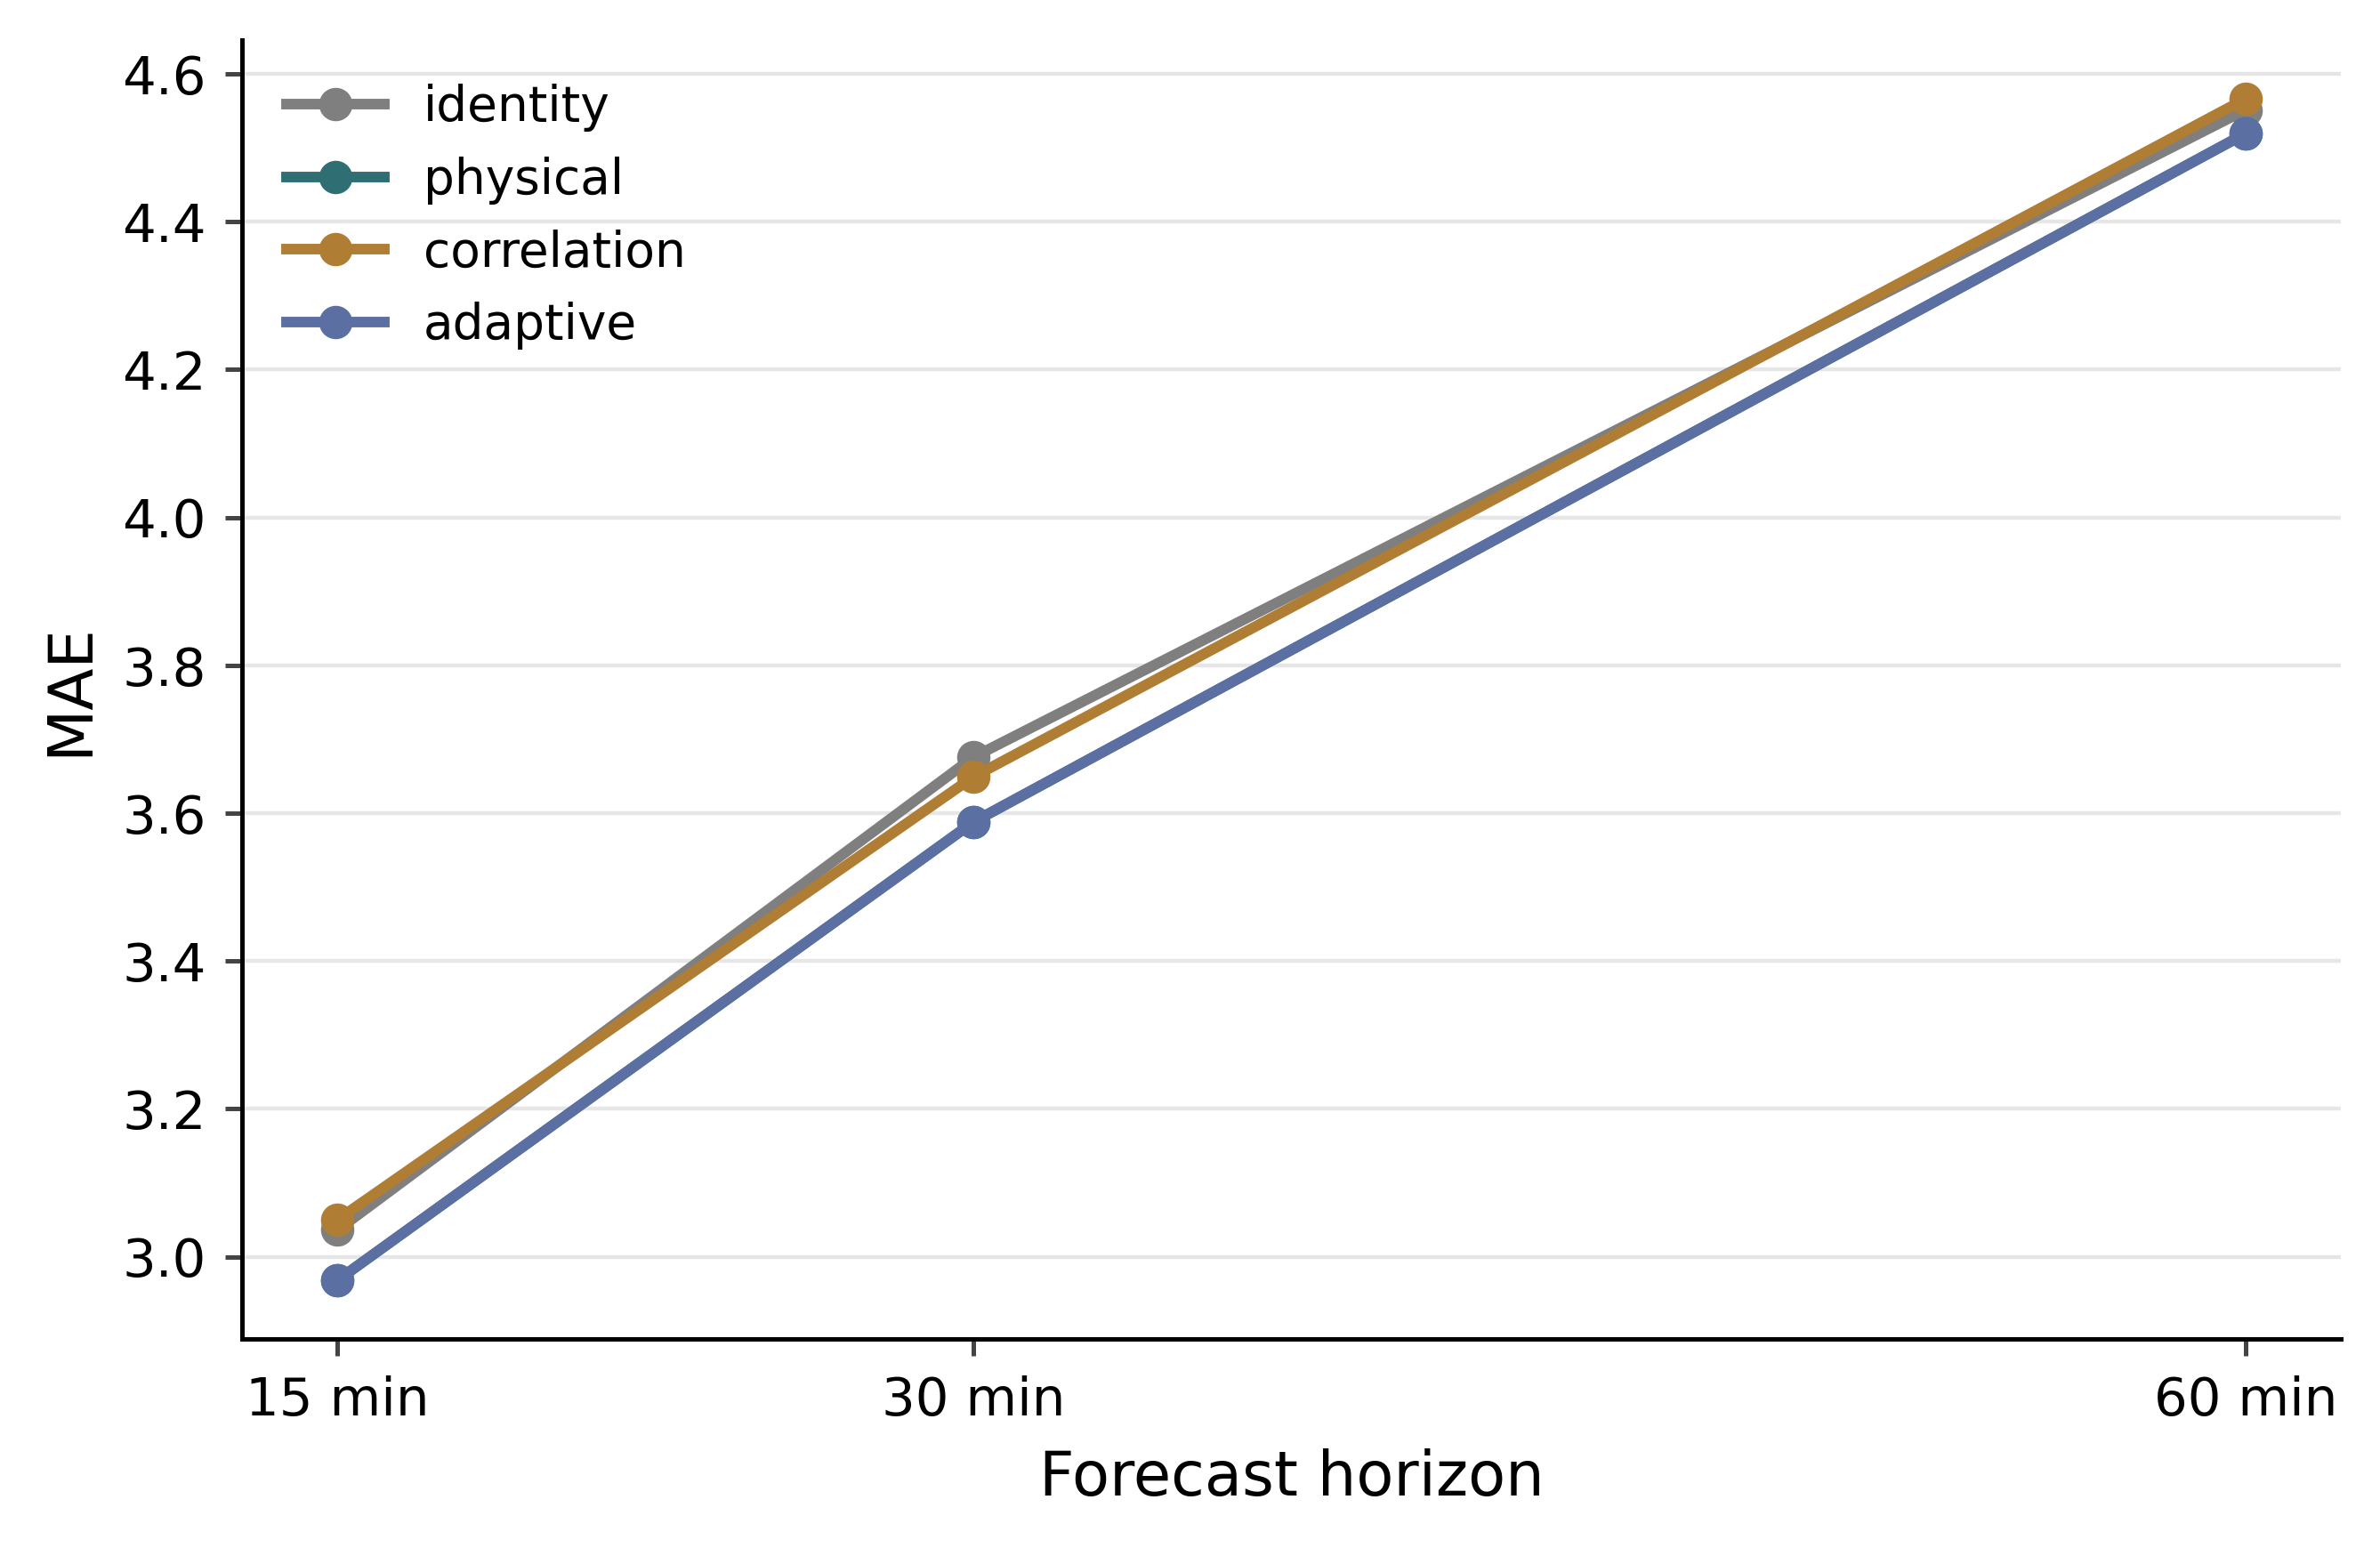
\includegraphics[width=0.82\linewidth]{../experiments/figures/GraphWaveNetFull_Graph_Ablation_MAE.png}
  \caption{GraphWaveNetFull ?????????}
  \label{fig:graph_ablation_cn}
\end{figure}

\section{????????}
??????????????????????????????? low speed?speed drop?high variance ? normal flow ?????Low speed ?????????speed drop ?????????????????high variance ?????????????normal flow ??????????????????

??????????? run ??GraphWaveNetFull ?????????? MAE??~\ref{tab:congestion_cn} ??? MAE ?????????????normal flow ???????? speed drop ? high variance ??????????????????????????????????

\begin{table}[htbp]
\centering
\caption{??? run ????????????}
\label{tab:congestion_cn}
\begin{tabular}{llrrr}
\toprule
?? & ???? & ???? & MAE & ??? \\
\midrule
Normal flow & GraphWaveNetFull & 30 ?? & 1.3958 & 3967395 \\
Low speed & GraphWaveNetFull & 15 ?? & 4.2541 & 901111 \\
Speed drop & GraphWaveNetFull & 15 ?? & 11.4046 & 275019 \\
High variance & GraphWaveNetFull & 15 ?? & 10.3429 & 459987 \\
\bottomrule
\end{tabular}
\end{table}

????????????? CSV ????????????? synthetic demo run??????????????????????? run??????????????? synthetic demo ??? run ????????

\begin{figure}[htbp]
  \centering
  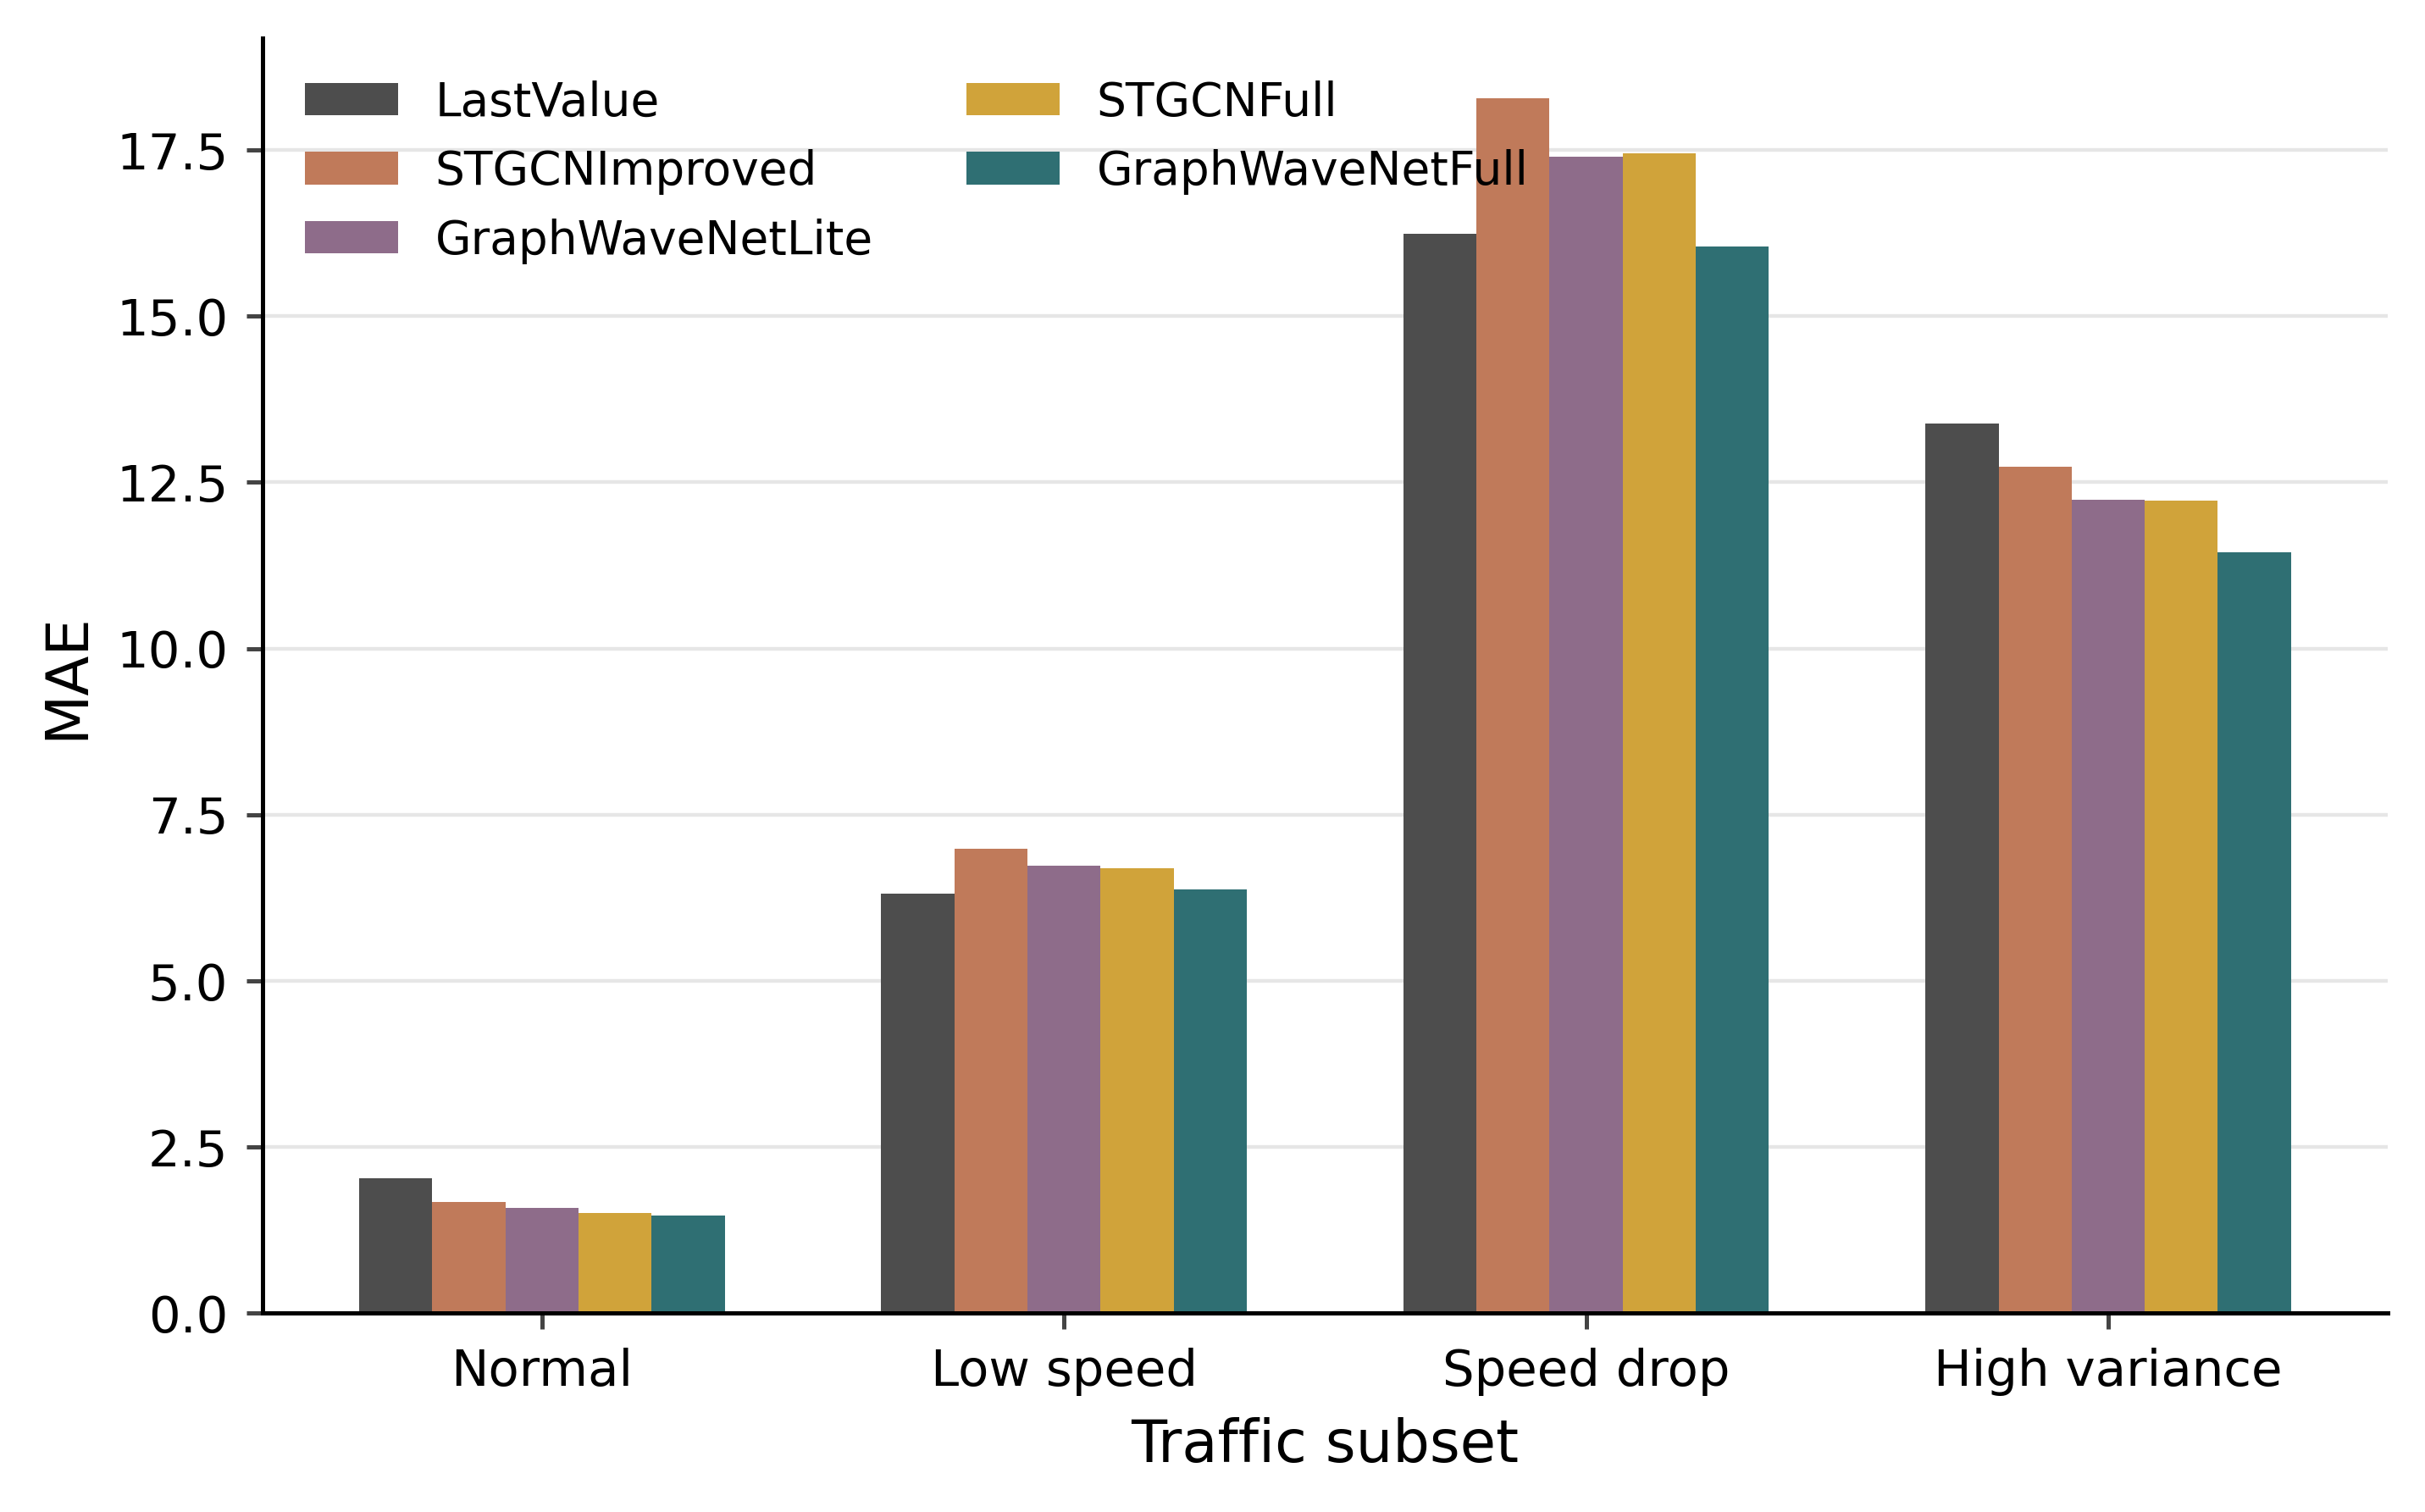
\includegraphics[width=0.82\linewidth]{../experiments/figures/Congestion_Subset_MAE_Main_Runs.png}
  \caption{??? run ???????? MAE?}
  \label{fig:congestion_subset_cn}
\end{figure}

\section{??????????}
GraphWaveNetFull ????? 0.73M?STGCNFull ?? 0.19M?GraphWaveNetLite ?? 0.057M?GraphWaveNetFull ???????????????????????????????????????????????????????????????????????????????????????????

\begin{figure}[htbp]
  \centering
  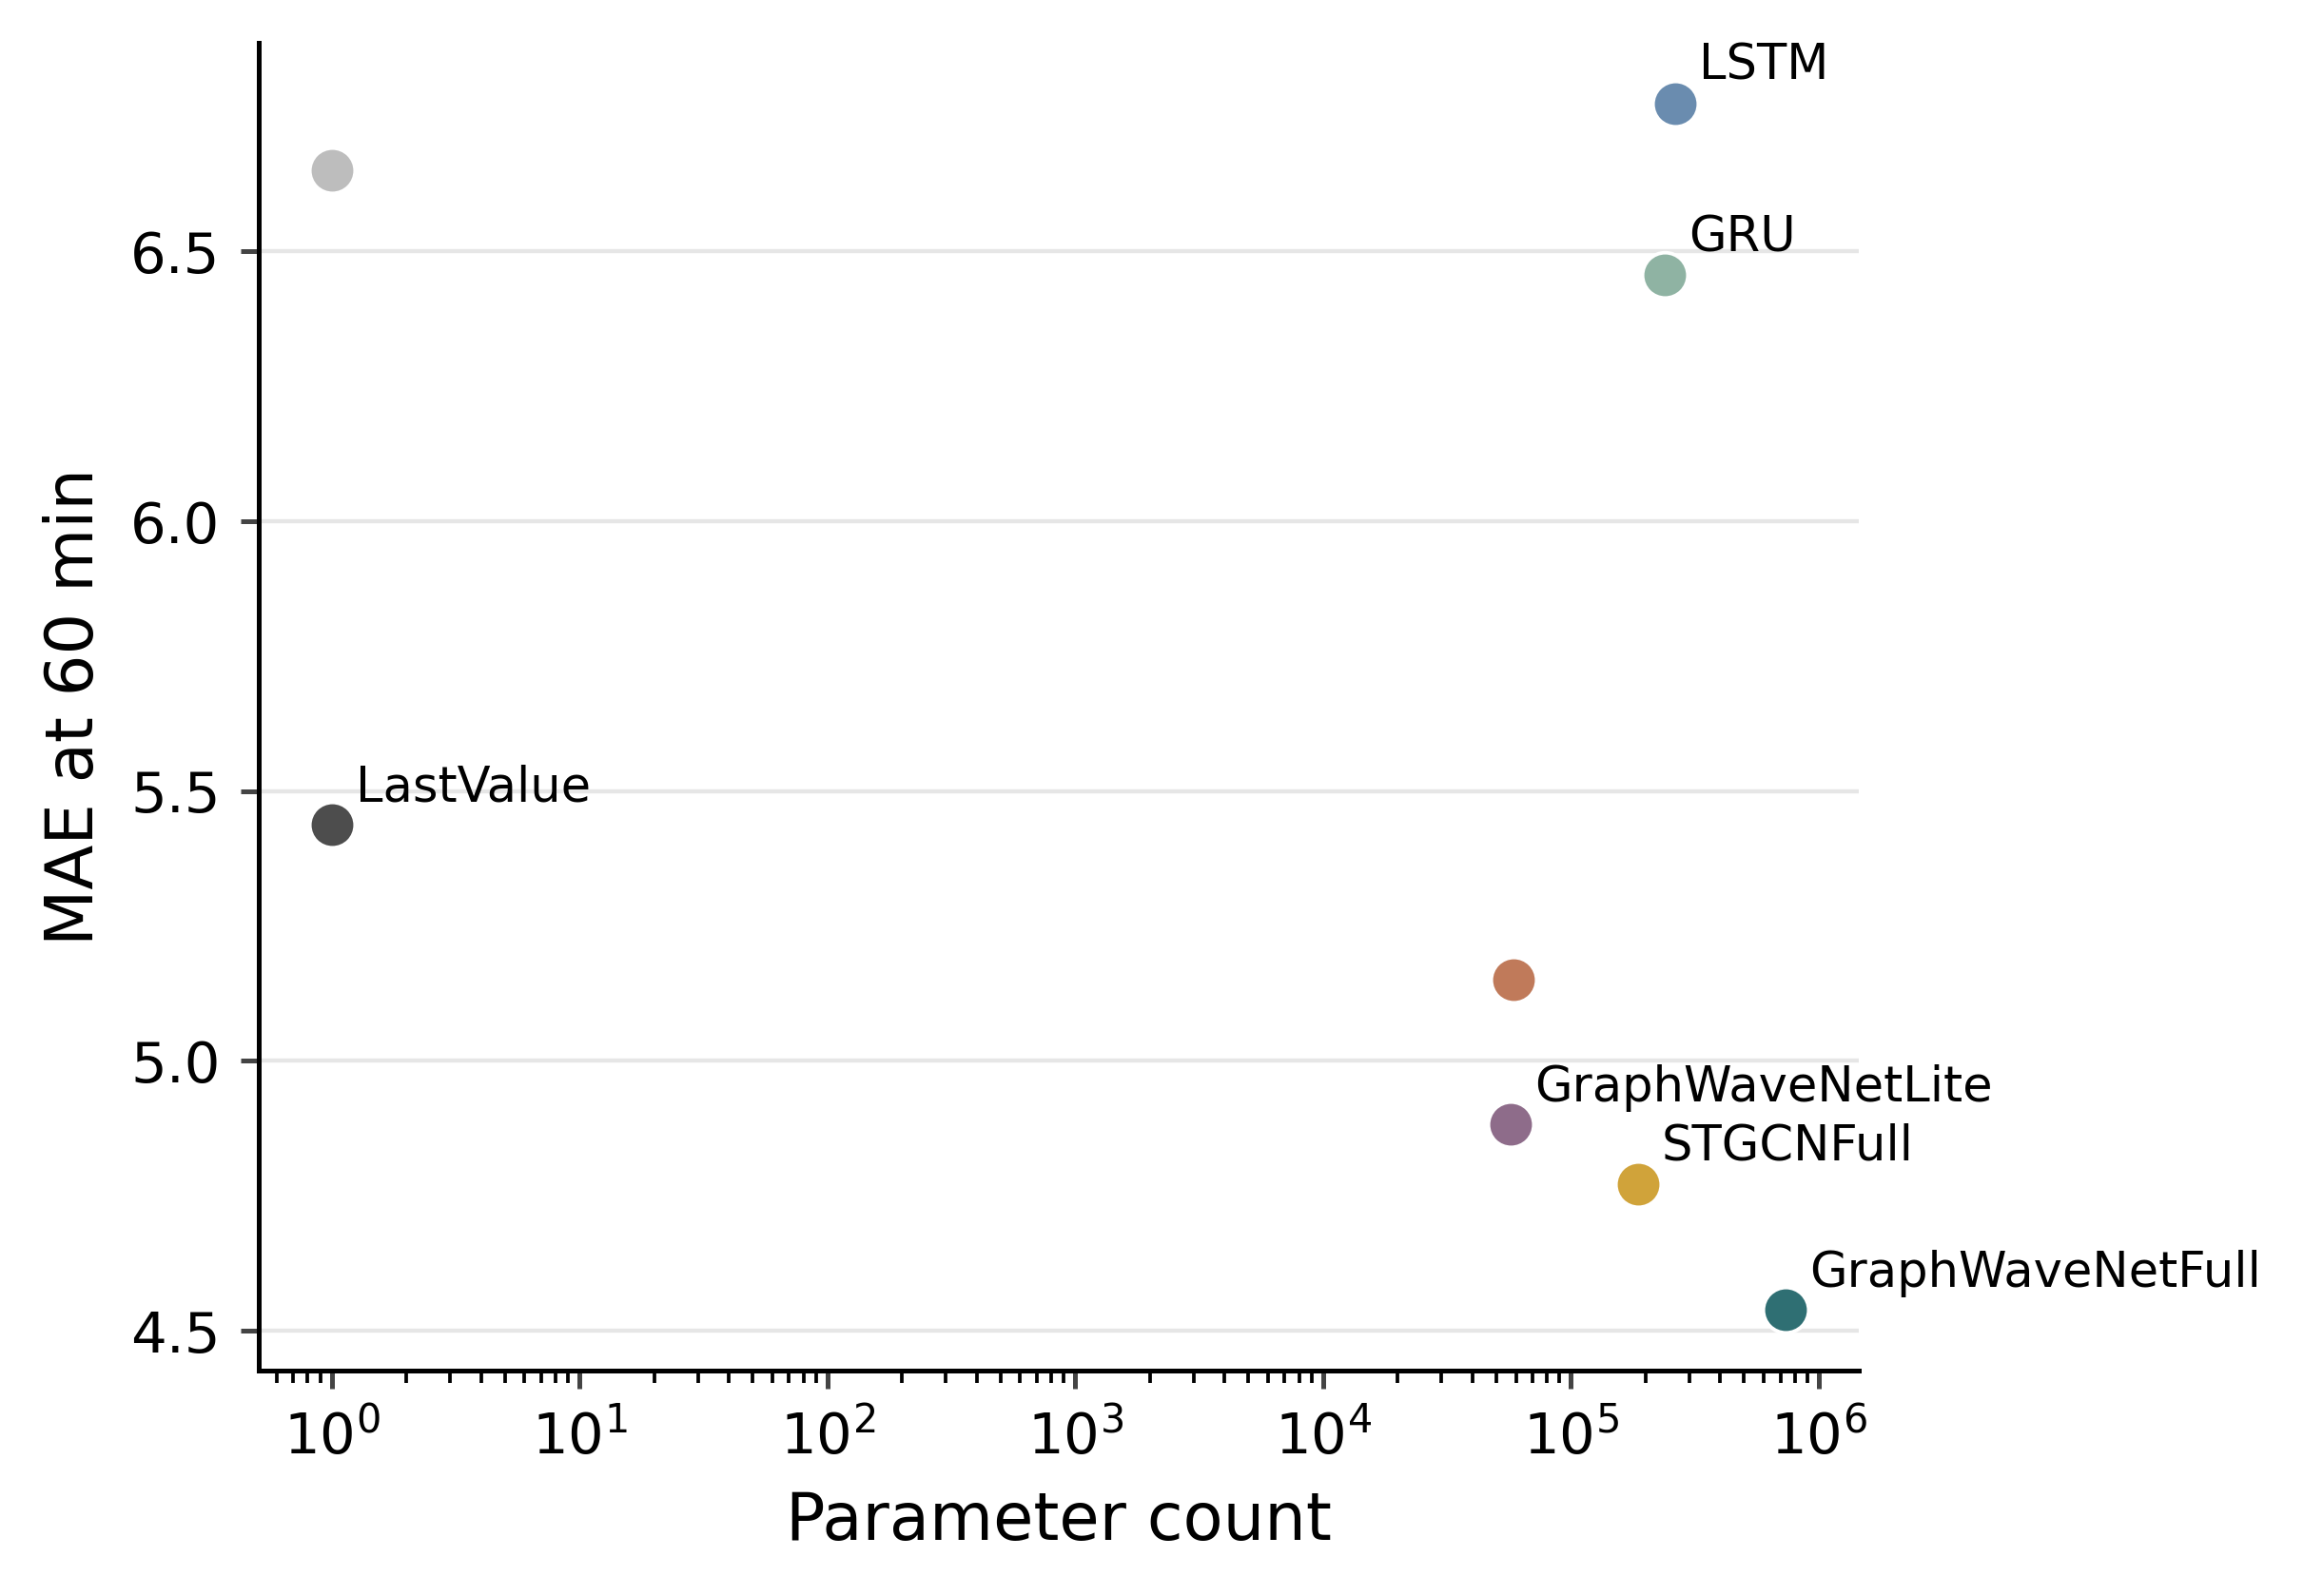
\includegraphics[width=0.78\linewidth]{../experiments/figures/Parameter_Count_vs_60min_MAE.png}
  \caption{???? 60 ?? MAE ????}
  \label{fig:param_tradeoff_cn}
\end{figure}

\section{??????????}
?? Agent ??????????????????????????????? trace ????????????? metrics??????????????????????????????????? LastValue???????????raw MAPE ????????????????????????????????????????????? outputs ????????

Agent ????????????????????????????????????????????????????????????????????

\section{??}
\subsection{LastValue ???}
?? GraphWaveNetFull ???????? LastValue?LastValue ????????????????????????????? 15 ???????????????????????? LastValue??????????????????? GraphWaveNetFull ??? horizon ???? LastValue???????????

\subsection{Raw MAPE ???}
Raw MAPE ??????? 0 ??????????????????????????????????????????????????????????? MAE?RMSE ? masked MAPE ???????

\subsection{????????}
??????? identity graph ???????????????????? physical graph?correlation graph ? adaptive graph ??????????????????????????????????????????????????????????????????????????????

\subsection{Full ???? Lite ?????}
GraphWaveNetFull ?? GraphWaveNetLite ????????????????????skip connection?? support ???? adaptive adjacency?STGCNFull ?? STGCNImproved ??????? ST-Conv block ?????????????????????????????????? full ???? lite ????????

\section{????????}
???????????????????? METR-LA ????????????????????????GraphWaveNetFull ? STGCNFull ? paper-inspired ???????????????????????????????????????????????????????????????????????????????????????????????????????????

\section{??}
????????????????????????????????????????????? seed ? horizon ?????????????????????????????? METR-LA ?????GraphWaveNetFull ? 15?30?60 ???????????? MAE?????? LastValue ?????????????????????????????????????? horizon????????????????????????????????????????

???????????? SOTA????????????????????????????????????? seed ??????????????????????????????????????????????????????

\appendix
\section{??????}
\begin{verbatim}
python -m traffic_agent.data.prepare_real_dataset \
  --dataset metr-la \
  --traffic-file data/raw/METR-LA/metr-la.h5 \
  --adj-file data/raw/METR-LA/adj_mx.pkl \
  --output data/processed/metr_la.npz

python -m traffic_agent.training.run_experiments \
  --config configs/metr_la_5090.yaml \
  --models last_value historical_average seasonal_naive gru lstm \
           stgcn_improved graph_wavenet_lite stgcn_full graph_wavenet_full \
  --horizons 3 6 12 \
  --seeds 42 43 44 \
  --output experiments/results/metr_la_5090_full_summary.csv

python -m traffic_agent.training.run_ablation \
  --config configs/metr_la_5090.yaml \
  --models stgcn_full graph_wavenet_full graph_wavenet_lite stgcn_improved \
  --horizons 3 6 12 \
  --seeds 42 43 44 \
  --graph-types identity physical correlation adaptive \
  --output experiments/results/metr_la_5090_ablation_summary.csv

python -m traffic_agent.analysis.congestion_eval \
  --runs-dir outputs \
  --output experiments/results/metr_la_congestion_subset_eval.csv
\end{verbatim}

\begin{thebibliography}{9}
\bibitem{li2018dcrnn}
Y. Li, R. Yu, C. Shahabi, and Y. Liu, ``Diffusion convolutional recurrent neural network: Data-driven traffic forecasting,'' in \emph{International Conference on Learning Representations}, 2018.

\bibitem{yu2018stgcn}
B. Yu, H. Yin, and Z. Zhu, ``Spatio-temporal graph convolutional networks: A deep learning framework for traffic forecasting,'' in \emph{International Joint Conference on Artificial Intelligence}, 2018.

\bibitem{wu2019graphwavenet}
Z. Wu, S. Pan, G. Long, J. Jiang, and C. Zhang, ``Graph WaveNet for deep spatial-temporal graph modeling,'' in \emph{International Joint Conference on Artificial Intelligence}, 2019.

\bibitem{kipf2017gcn}
T. N. Kipf and M. Welling, ``Semi-supervised classification with graph convolutional networks,'' in \emph{International Conference on Learning Representations}, 2017.

\bibitem{hochreiter1997lstm}
S. Hochreiter and J. Schmidhuber, ``Long short-term memory,'' \emph{Neural Computation}, vol. 9, no. 8, pp. 1735--1780, 1997.

\bibitem{cho2014gru}
K. Cho et al., ``Learning phrase representations using RNN encoder--decoder for statistical machine translation,'' in \emph{Conference on Empirical Methods in Natural Language Processing}, 2014.
\end{thebibliography}

\end{document}
